% mnras_template.tex 
%
% LaTeX template for creating an MNRAS paper
%
% v3.0 released 14 May 2015
% (version numbers match those of mnras.cls)
%
% Copyright (C) Royal Astronomical Society 2015
% Authors:
% Keith T. Smith (Royal Astronomical Society)

% Change log
%
% v3.0 May 2015
%    Renamed to match the new package name
%    Version number matches mnras.cls
%    A few minor tweaks to wording
% v1.0 September 2013
%    Beta testing only - never publicly released
%    First version: a simple (ish) template for creating an MNRAS paper

%%%%%%%%%%%%%%%%%%%%%%%%%%%%%%%%%%%%%%%%%%%%%%%%%%
% Basic setup. Most papers should leave these options alone.
\documentclass[fleqn,usenatbib,]{mnras}
\usepackage{lineno}
\linenumbers
% MNRAS is set in Times font. If you don't have this installed (most LaTeX
% installations will be fine) or prefer the old Computer Modern fonts, comment
% out the following line
\usepackage{newtxtext,newtxmath}
% Depending on your LaTeX fonts installation, you might get better results with one of these:
%\usepackage{mathptmx}
%\usepackage{txfonts}

% Use vector fonts, so it zooms properly in on-screen viewing software
% Don't change these lines unless you know what you are doing
\usepackage[T1]{fontenc}
\usepackage{ae,aecompl}


%%%%% AUTHORS - PLACE YOUR OWN PACKAGES HERE %%%%%

% Only include extra packages if you really need them. Common packages are:
\usepackage{graphicx}	% Including figure files
\usepackage{amsmath}	% Advanced maths commands
\usepackage{amssymb}	% Extra maths symbols
\usepackage{booktabs}   % Make tables directly in pandas
\usepackage{longtable}  % Add longer tables
\usepackage{rotating}
\usepackage{appendix}
\usepackage{float}
\usepackage[dvipsnames]{xcolor}
\usepackage{subcaption}
\usepackage{multicol}
\usepackage{wrapfig}
\PassOptionsToPackage{hyphens}{url}\usepackage{hyperref}
\captionsetup{compatibility=false}

\setlength{\rotFPtop}{0pt plus 1fil}% <- add this line after loading rotating
\setlength{\rotFPbot}{0pt plus 1fil}% <- maybe its better to add this line too
\usepackage{threeparttable}
\makeatletter
%\newlength{\abovecaptionskip}%
%\setlength{\abovecaptionskip}{10\p@}
\makeatother
\usepackage{booktabs}
%%%%%%%%%%%%%%%%%%%%%%%%%%%%%%%%%%%%%%%%%%%%%%%%%%

%%%%% AUTHORS - PLACE YOUR OWN COMMANDS HERE %%%%%

% Please keep new commands to a minimum, and use \newcommand not \def to avoid
% overwriting existing commands. Example:
%\newcommand{\pcm}{\,cm$^{-2}$}	% per cm-squared
%Co-authors:
\newcommand{\phil}[1]{\color{red}#1 \color{black}}

\newcommand{\comment}[1]{\textbf{[#1]}} %comments

%define some nice astro shortcuts
\newcommand{\halpha}[0]{H$\alpha$}
\newcommand{\hbeta}[0]{H$\beta$}
\newcommand{\OII}[0]{$[\textnormal{\textsc{Oii}}]$}
\newcommand{\OIII}[0]{$[\textnormal{\textsc{Oiii}}]$}
\newcommand{\SII}[0]{$[\textnormal{\textsc{Sii}}]$}
\newcommand{\SIII}[0]{$[\textnormal{\textsc{Siii}}]$}
\newcommand{\NII}[0]{$[\textnormal{\textsc{Nii}}]$}
\newcommand{\msun}[0]{M_{\odot}}


\defcitealias{Pursiainen2018}{P18}
\defcitealias{Pursiainen2020}{P20}
%%%%%%%%%%%%%%%%%%%%%%%%%%%%%%%%%%%%%%%%%%%%%%%%%%
%This if a fix from https://tex.stackexchange.com/questions/249579/pdfendlink-ended-up-in-different-nesting-level-than-pdfstartlink-error-with/249743#249743 to sort hyperref breaking in pdfendlink when a reference spills over a page
%\usepackage{etoolbox}
%\makeatletter
%\patchcmd\@combinedblfloats{\box\@outputbox}{\unvbox\@outputbox}{}{%
%  \errmessage{\noexpand\@combinedblfloats could not be patched}%
%}%
%\makeatother
%
%\defcitealias{Smith2019}{S19}
%\defcitealias{Kelly2012}{KK12}
%%%%%%%%%%%%%%%%%%% TITLE PAGE %%%%%%%%%%%%%%%%%%%

% Title of the paper, and the short title which is used in the headers.
% Keep the title short and informative.
\title[Supernova hosts in DES]{Supernova Host Galaxies in the Dark Energy Survey: \\ II. Rapidly Evolving Transients}
% The list of authors, and the short list which is used in the headers.
% If you need two or more lines of authors, add an extra line using \newauthor
\author[P. Wiseman et al.]{
P. Wiseman$^1$\thanks{E-mail: p.s.wiseman@soton.ac.uk (PW)},
 M. Pursiainen$^1$,
 M. J. Childress$^1$,
 M. Smith$^1$,
 and Other Authors$^{1,2}$,
\newauthor
(The DES Collaboration)
\\
% List of institutions
$^{1}$School of Physics and Astronomy, University of Southampton, Southampton, SO17 1BJ, UK\\
$^{2}$Other Institutions\\
%$^{3}$Another Department, Different Institution, Street Address, City Postal Code, Country
}

% These dates will be filled out by the publisher
\date{Accepted XXX. Received YYY; in original form ZZZ}

% Enter the current year, for the copyright statements etc.
\pubyear{2020}
% These dates will be filled out by the publisher

% Don't change these lines
\begin{document}
\label{firstpage}
\pagerange{\pageref{firstpage}--\pageref{lastpage}}
\maketitle

% Abstract of the paper
\begin{abstract}
Rapidly evolving transients (RETs) are a mysterious class of astrophysical event. They are characterised by lightcurves that decline much faster than standard supernovae (SNe), span vast ranges in peak luminosity and can be seen to redshifts greater than 1. Their evolution on fast timescales has hindered high quality follow-up observations, such that their origin and explosion/emission mechanism remains unexplained. In this paper, we investigate the host galaxies of the largest RET sample to date from the Dark Energy Survey (DES). Using deep-stacked photometry and emission-lines from OzDES spectroscopy, we derive host galaxy stellar mass, star-formation rate (SFR), and metallicity for 42 hosts. We find that RETs explode almost exclusively in star-forming galaxies and are thus likely associated with massive stars. Comparing RET hosts to samples of host galaxies of other explosive transient as well as field galaxies, we find that RETs prefer galaxies with high specific SFR, indicating a link to young stellar populations stripped-envelope SNe. RET hosts appear to show a lack of chemical enrichment, their metallicities akin to long duration gamma-ray bursts and superluminous SNe host galaxies. 

\end{abstract}

% Select between one and six entries from the list of approved keywords.
% Don't make up new ones.
\begin{keywords}
keyword1 -- keyword2 -- keyword3
\end{keywords}

%%%%%%%%%%%%%%%%%%%%%%%%%%%%%%%%%%%%%%%%%%%%%%%%%%

%%%%%%%%%%%%%%%%% BODY OF PAPER %%%%%%%%%%%%%%%%%%

\section{Introduction}



In the standard paradigm of stellar evolution, stars with a zero-age main sequence (ZAMS) mass above $8M_{\sun}$ are believed to explode as a result of a catastrophic collapse of their iron cores and are known as core-collapse supernovae (CCSNe). CCSNe can be split into observationally-determinded subclasses based on their lightcurve and spectral evolution: SNe II display hydrogen features in their spectra, and are thought to occur in stars that retain a large fraction of their hydrogen envelope. Conversely, SNe Ib and Ic do not show signatures of hydrogen and are thus referred to collectively as stripped-envelope SNe (SESNe). The SN IIb subclass, which shows hydrogen only at early epochs, is also commonly grouped along with SESNe. Since the turn of the century, observations of CCSNe, whose lightcurves are primarily powered by the radioactive decay of freshly synthesised Ni-56, have been supplemented by rarer, more exotic transient classes.

 Long duration gamma-ray bursts (LGRBs), although first discovered in the 1960s \citep{Klebesadel1973} were only unequivocally linked to collapsing massive stars through their associations with broad-lined type Ic SNe \citep{Galama1998,Hjorth2003}. Thought to be caused by accretion onto a newly-formed black hole at the centre of a collapsing, rapidly-rotating massive star \citep[e.g.][]{Woosley1993,Woosley2006a,Woosley2006b}, LGRBs comprise roughly $1\%$ of all SNe Ic, themselves making up only 15\% of all CCSNe \citep{Kelly2012,Graham2016}. The second exotic class of SNe is the particularly bright superluminous supernovae (SLSNe; e.g. \citealt{Quimby2011, Gal-Yam2012}). Originally grouped due to their slowly-evolving lightcurves and extreme luminosity (peaking at $M_B < -21$~mag; 10-100 times brighter than regular CCSNe), recent observations have revealed a continuum of spectroscopically similar objects with peaks as faint as $M_B \sim -19$~mag \citep{DeCia2018,Lunnan2018,Angus2019}, similar to the bright end of the CCSN luminosity function \citet{Li2011,Grayling2020}. The lightcurve evolution of SLSNe is not well described by models of Ni-56 decay, with the most popular alternative hypothesis being the magnetic coupling of the ejecta with the spin down of a newly formed, rapidly rotating magnetar.
 
 Along with observations of the transients themselves, host galaxies are frequently-used laboratories from which strong inferences about the progenitor stars and explosion mechanisms can be made. CCSNe are confined almost exclusively to galaxies hosting recent or ongoing star formation, due to their origin from massive stars. There are correlations between the expected progenitor mass of different sub-classes of CCSNe and host galaxy properties. On average, SESNe reside in galaxies with higher specific star-formation rate (sSFR) and younger stellar age indicating that their progenitors are more massive than the various sub-classes of hydrogen-rich SNe II \citep{James2006,Kelly2008,Galbany2018}. More extreme events tend to occur in galaxies low in mass and high in sSFR, with both GRBs \citep[e.g.][]{Fruchter2006,LeFloch2006,Levesque2010,Kruehler2015,Vergani2015,Perley2016b,Palmerio2019,Taggart2019} and to an even greater degree SLSNe \citep[e.g.][]{Neill2011,Lunnan2014,Leloudas2015,Angus2016,Schulze2018,Taggart2019} exhibiting this association.
 
 The chemical composition of the interstellar medium (ISM) is an important consideration when comparing host galaxy properties. While it does not appear to play a significant role in the relative production of CCSNe (although there are some trends, with SESNe typically found in slightly less metal-rich galaxies than SNe II; \citealt{Galbany2018}), it appears to be vitally important in the production of LGRBs and SLSNe. Theory predicts that the production of a LGRB should only be possible in stars with a metallicity of $Z/Z_{\sun}\leq 0.3$ \citep{Woosley1993}  in order for the likely Wolf-Rayet or blue supergiants progenitors not to lose their outer atmospheres through metal-driven winds, thus conserving sufficient angular momentum to power the black-hole-driven jet or rapidly rotating magnetar. Many LGRB host galaxy studies have indeed revealed a metallicity threshold to be observed between 0.5 and 1 times the solar value \citep[e.g.][]{Stanek2006,Modjaz2008,Kruehler2015,Perley2016b,Japelj2016,Vergani2017}.  
SLSN host galaxies also appear to be lower in metallicity than would be expected for their stellar mass, with a suppression of SLSN production at a value around half-solar \citep{Lunnan2014,Chen2016a,Perley2016c}. They also require particularly high sSFR, suggesting that they are explosions of very young, rapidly rotating massive stars.
 
Recently, inspection of high-cadence, all-sky survey data sets have revealed yet more exotic transients that are less easy to explain with conventional models. \citet{Drout2014} revealed a class of rapidly evolving transients (RETs; also termed `Fast Blue Optical Transients' - FBOTs or `Fast Evolving Luminous Transients' - FELTs) in the Pan-STARRS survey (PS1). \citet{Pursiainen2018} expanded the known number of RETs to beyond 80 with their sample from the Dark Energy Survey (DES), spanning a redshift range of $\sim 0$ to $>1$. RETs typically rise to peak brightness within 7-10 days, and decline to 10\% of their peak brightness within 30 days, much faster than typical SNe. The photometric measurements of the PS1 and DES RETs seem to be well described by simple expanding blackbodies, although a handful show declining photospheric radii from the outset. Due to the rapid nature of their lightcurves and location at high-redshift, spectral coverage is sparse and signal-to-noise ratio (SNR) is low, such that there has not yet been a conclusive detection of absorption or emission features from the transients and thus the physical mechanism responsible for their rapid evolution remains unexplained.

There are a limited number of events detected in the local Universe whose properties are consistent with the RETs seen in the samples of PS1 and DES at cosmological distances, the most widely studied of which is AT2018cow \citep[e.g.][]{Prentice2018,Perley2019}. The transient declined from its discovery, with constraints on a ~1 day rise time, and across the full range of observed wavelengths did not resemble any known SN, GRB afterglow, or kilonova (KN) \citep{Ho2019}. There are myriad explanations for the power source of AT2018cow touted in the literature, including: magnetars \citep{Mohan2020}; electron capture collapse of merged white dwarfs \citep{Lyutikov2019}; a tidal disruption event (TDE) of a white dwarf \citep{Kuin2019} or of a main sequence star by an intermediate mass black hole \citep{Perley2019}; common envelope jets supernova (CEJSN) \citep{Soker2019}
Other nearby rapid transients include the local fast-declining SN-like transient \citep{McBrien2019} which is explained by the destruction of a white dwarf in a non-standard scenario, and KSN-2015K \citep{Rest2018} whose fast rise and decline is explained by the shock of an SN running into previously-expelled material.  It is currently unclear whether these transients do indeed represent the local analogues of the DES and PS RETs.

In this paper, we present the first comprehensive study of the host galaxies of RETs. We make use of the final DES sample, which builds on \citet{Pursiainen2018} using the final year of data as well as more refined discovery techniques. Using the deep DES photometry from \citet{Wiseman2020} and spectra from OzDES \citep{Lidman2020} we derive host galaxy properties in order to compare them to samples of CCSNe, LGRBs, and SLSNe, as well as the individual local rapid transients. For clarity, we will use the term RET to refer only to events in the high-redshift samples of DES and PS1. 

The order of the paper is as follows:
Where applicable, we adopt a spatially flat $\Lambda$CDM cosmology with the parameters H$0=70$ km~s$^{-1}$ and $\Omega_{\textrm{M}}=0.3$.


\begin{figure*}
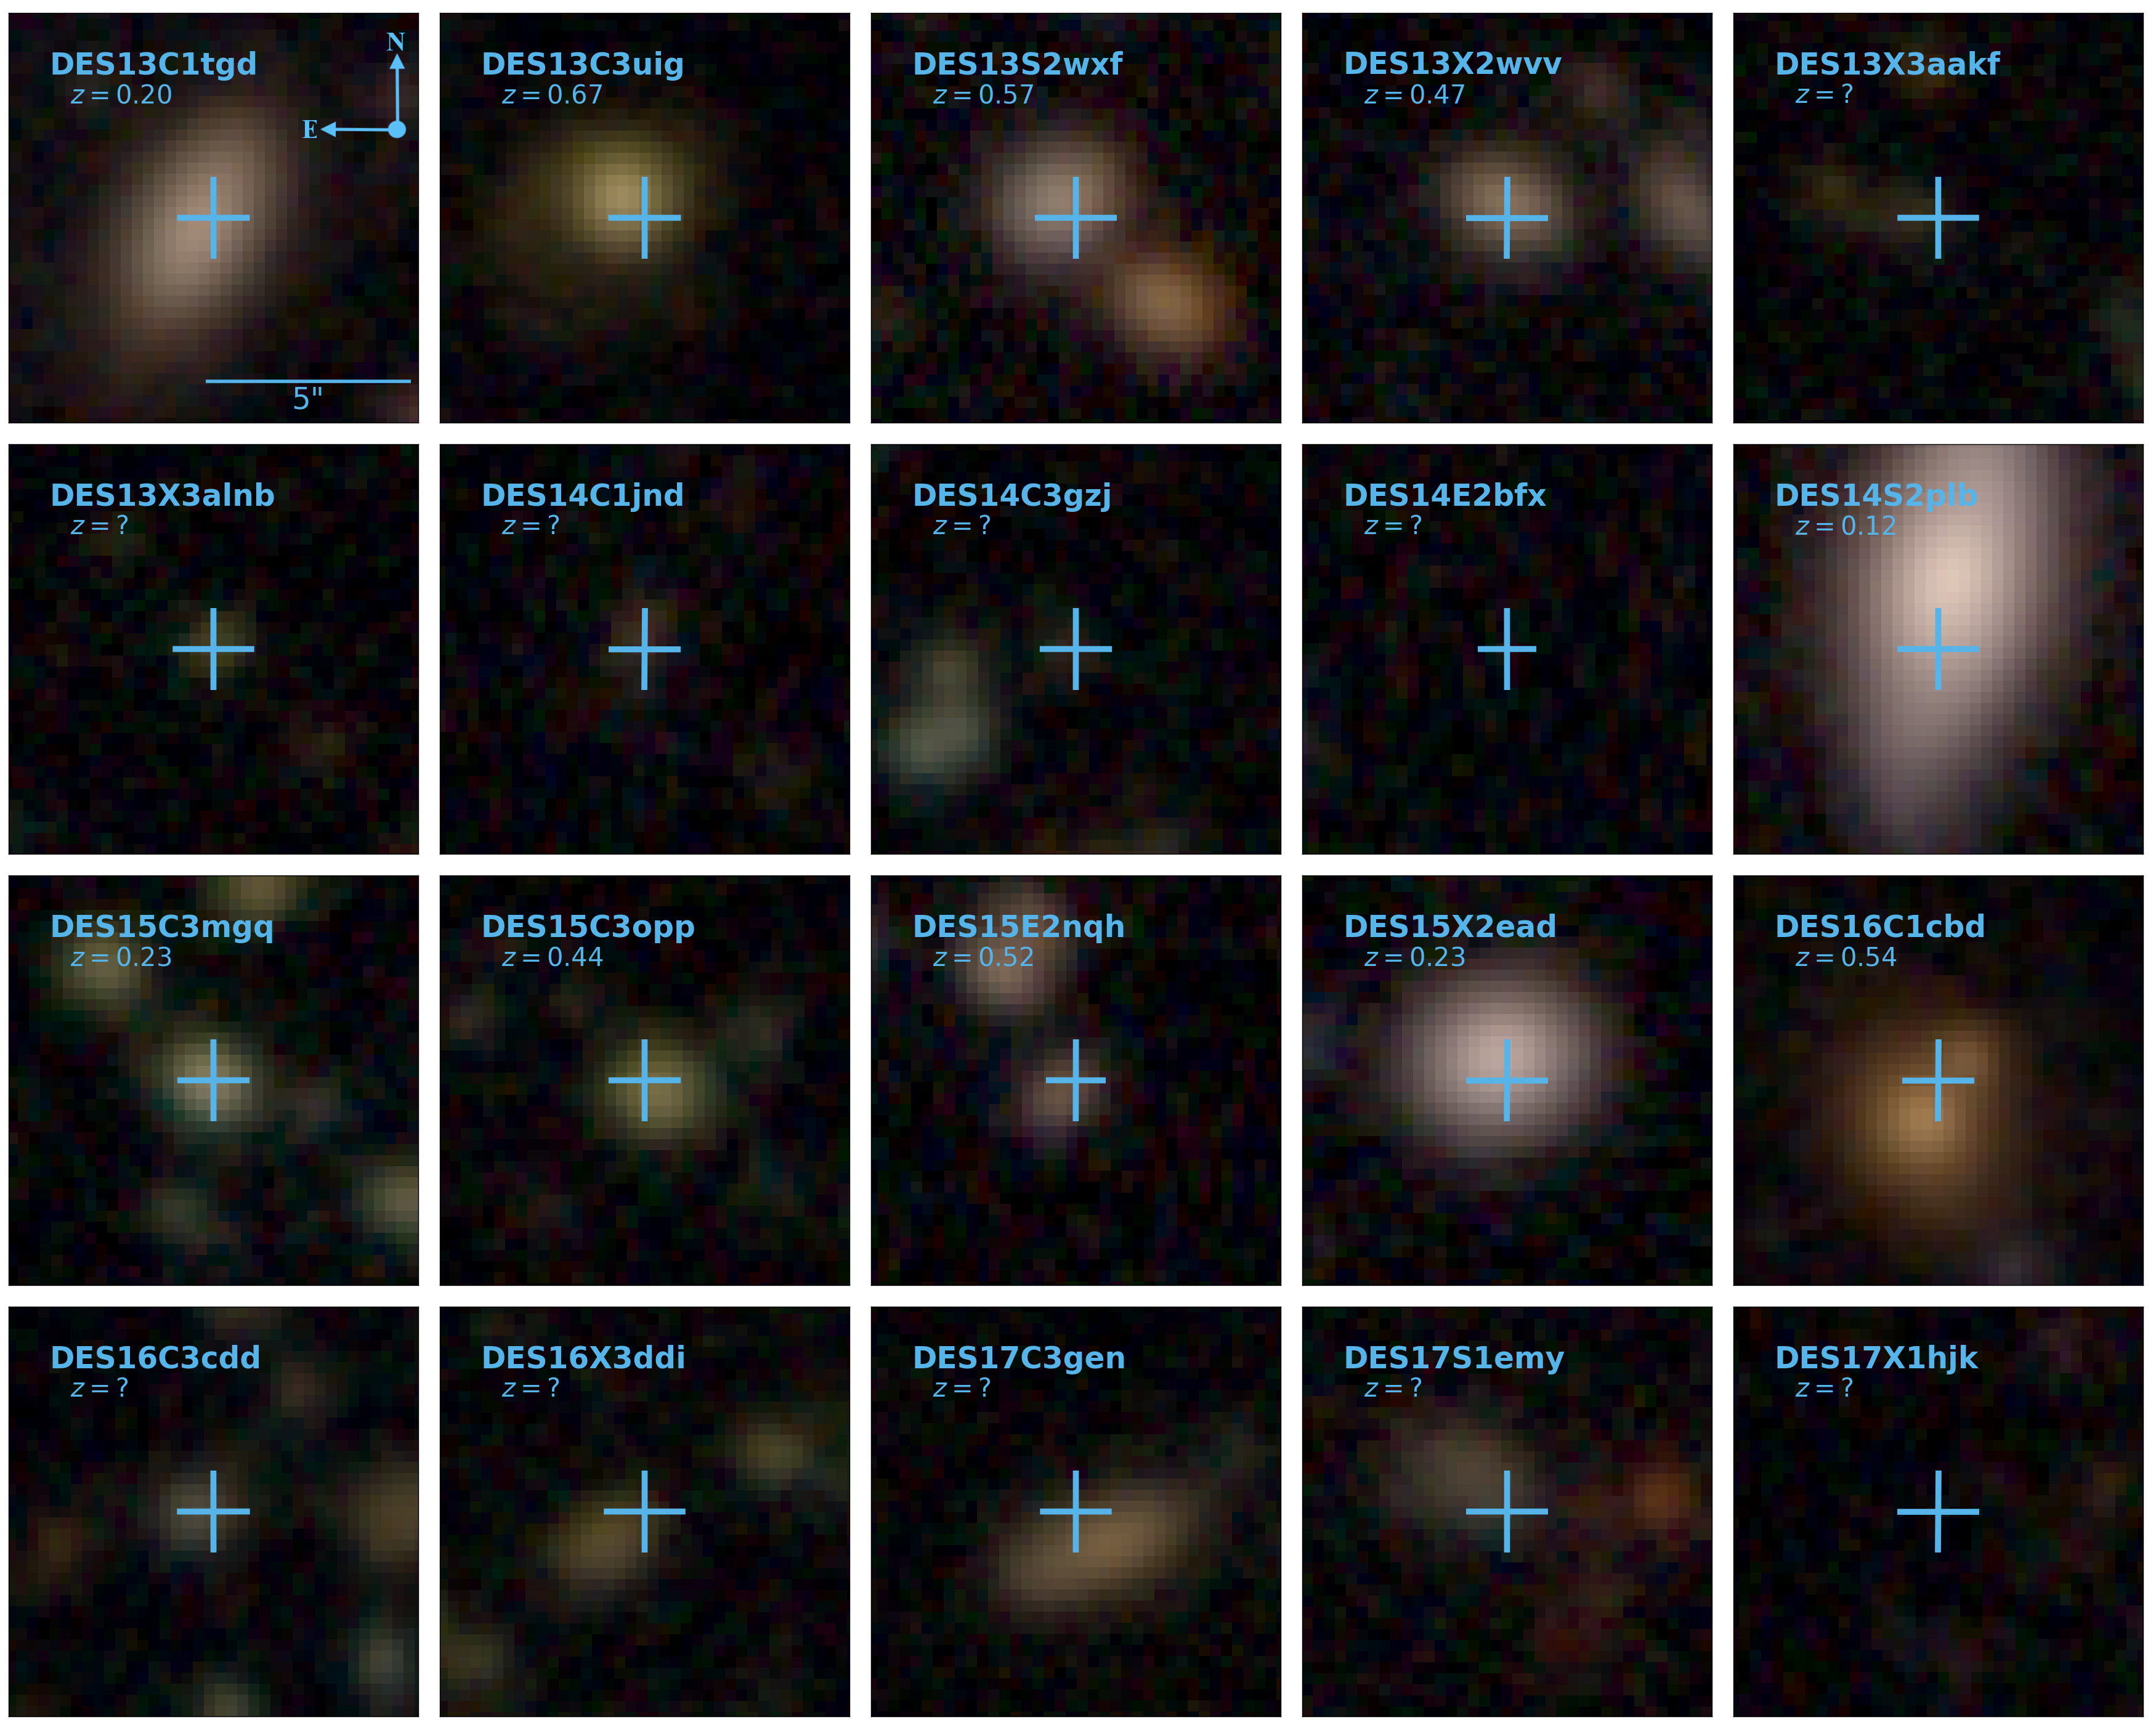
\includegraphics[width=\textwidth]{figs/RET_Mosaic.png}
\caption{Selection of DES RET host galaxies in an RGB composite of the DES $gri$ bands. The locations of the transients are indicated with cyan crosses.
\label{fig:mag_dist}}
\end{figure*}

\begin{figure}
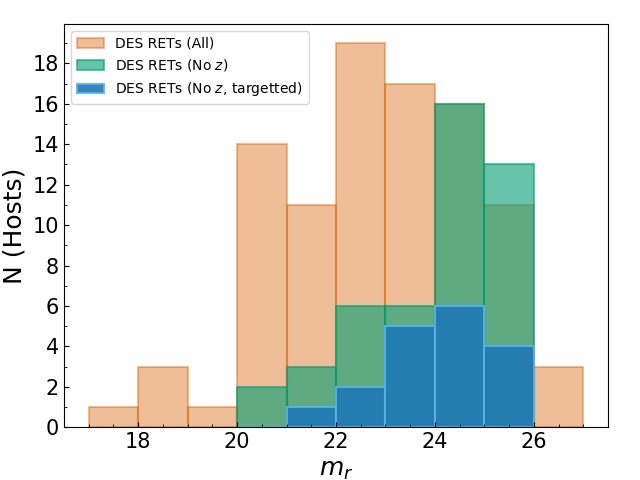
\includegraphics[width=0.5\textwidth]{figs/mag_dist.png}
\caption{Observer-frame $r$-band magnitude distribution for the host galaxies of RETs in DES. The orange histogram represents the 97/106 DES RETs for which a host was detected. The green histogram shows those that did not have a successful redshift measurement, while blue shows those with no redshift despite being targetted by OzDES.
\label{fig:mag_dist}}
\end{figure}

\begin{figure}
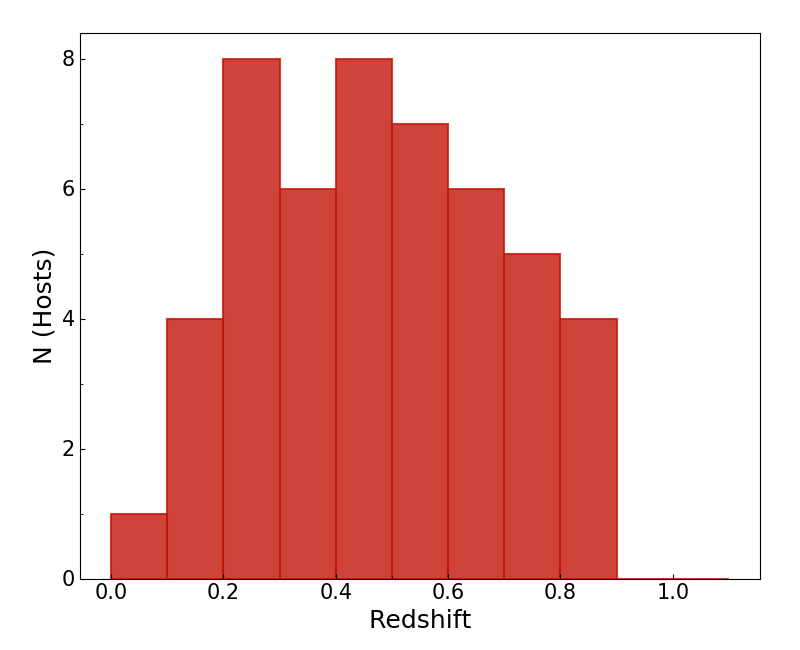
\includegraphics[width=0.5\textwidth]{figs/z_dist.png}
\caption{Redshift distribution for the host galaxies of RETs in DES for which a measurement was obtained.
\label{fig:z_dist}}
\end{figure}

\section{Sample selection\label{sec:sample}}

We derive our sample from the 106 RETs discovered in the 5-year DES-SN transient survey. This number expands upon the 72 of \citetalias{Pursiainen2018}. The first reason for the increased sample size is the use of the 5th year of DES-SN, where \citetalias{Pursiainen2018} were only able to make use of the first four years. The second reason is an update to the sample selection technique. By imposing the \citetalias{Pursiainen2018} selection criteria on season 5, the sample is increased to 96 objects.

\subsection{Improvements to the search method}

The original method of finding RETs in the DES-SN data (and presented in \citetalias{Pursiainen2018}) was designed to be simple and used light curve modelling with Gaussian and linear fits. The simplistic method made it possible to look for exotic transients without knowing their observed characteristics beforehand and resulted in a large sample of photometrically selected fast transients. However, as the search was simplistic and relied heavily on visual inspection of the available data (etc. images, light curves, host galaxy information), it is impossible to be sure how complete the sample is. For instance, due to the large redshift range within the sample it is entirely possible that distant events could have been missed due to time dilation. Here, a more sophisticated search method is presented. As only a fraction of transients in DES-SN have redshift information from host galaxy, the search must be done in the observer frame.  The key features of RETs that distinguishes them from most traditional SNe types are the fast light curve evolution and blue colour at peak. Even though both of these quantities depend on the redshift of the transient, they still seem to distinguish the the fast events from traditional SN types. 

To assess the distinguishing photometric properties of RETs, we take the sample of 72 from the \citetalias{Pursiainen2018} method along with spectroscopically confirmed SNe of types Ia, Ibc, II, and SLSNe from DES that pass the following criteria:
\begin{enumerate}
\item The transient was only detected in one DES-SN observing season.
\item Maximum observed brightness in both $g$- and $r$-bands was brighter than 24 mag (in the eight `shallow' DES-SN fields) or 25 mag (in the two `deep' fields).
\item $g$- and $r$-band observations used for the colour had to be taken within 2 days in observer frame.
\end{enumerate}

Of objects passing these cuts, the RETs cluster at shorter timescales and bluer colours than other SNe, even in the observer frame. However, using photometric data points directly has several problems that can be improved. For one, measuring peak colour is problematic: DES-SN did not always observe $g$- and $r$-bands on the same or even consecutive nights, thus making it impossible to measure the peak colour in a number of cases. Measuring rise times of 10-15 days is difficult to perform with a one week cadence when it has to be done without fitting a light curve model, hence the rise time values are spread over a wide range. To negate this issue, we interpolate the light curves using the method of Gaussian processes (GP). The interpolated light curves have a 0.5 day cadence and every epoch has a flux value, and an associated uncertainty, for each band. Using this technique, SNe Ia and RETs populate two distinct regions of $g-r$-$t_{\mathrm{rise; r}}$ parameter space and are thus easier to separate. We define a region in this parameter space which minimises the contamination of non-RETs (purity) while maximising the total fraction of RETs (completeness). The resulting limits are $-1.5 < g-r < 0.6 $ and $t_{\mathrm{rise; r}} <16.5$.

We process all $\sim 30,000$ DES-SN transient candidates with GP. In order to reduce the contamination from active galactic nuclei (AGN), we use a basic convolutional neural network (CNN) classifier which we train on spectrosopically confirmed objects, and use to separate the sample into two subtypes: AGN-like and SNe-like. The classifier returns SNe-like objects with an accuracy of 0.992 on the test set; the remaining AGN are likely removed by the final manual vetting.
The SNe passing the CNN classifier are subjected to the LC quality cuts, resulting in 2259 objects, of which 939 lie inside the colour and rise-time region which we defined as RETs. These objects are subject to a further set of cuts. We impose a cut based on a fit of the LC with the \texttt{PSNID} software (\citet{Sako2008}). We use thresholds of \texttt{FITPROB}$<0.91$ and \texttt{PBAYES}$<0.82$ to remove highly-probably SNe Ia, which removes 46 objects from the RET parameter space. In order to further remove longer-lived SNe, the decline time to half of the peak brightness must be $<24$ days. This removes 347 SNe, resulting in 546 objects remaining inside the parameter space. The final 564 transients have been visually inspected, with the majority rejected for being spurious detections, obvious multi-season variability that was not picked up by the CNN, or showing evidence for a longer timescale decline. 

Using the above method recovers N of the 96 rets found using the \citetalias{Pursiainen2018} technique, and adds a further M.
We refer to the resulting sample as DES RETs. Of the 106 objects in the sample, 97 have a host galaxy detected in deep host galaxy photometry of \citet{Wiseman2020}, of which 49 have a host galaxy spectroscopic redshift. A further three have redshifts obtained from narrow lines observed in spectra of the transients themselves. We do not consider these three objects for the analysis, since we are unable to separate transient and host contributions to the spectra.

\subsection{Comparison samples \label{subsec:comparison}}

In order to compare the host galaxies of DES RETs to those discovered in other surveys as well as other types of explosive transient, we draw upon samples in the literature. 

\subsubsection{RETs \label{subsubsec:compare_rets}}
Since the DES sample of RETs is by far the largest discovered to date, there is no other large sample of RETs with which to compare host galaxy properties. \citet{Drout2014} present host galaxies of 10 RETs discovered in the Pan-STARRS survey, with measurements of stellar masses and SFRs. To this we add the low-redshift transients AT2018cow \citep[e.g.][], with host galaxy measurements from \citet{Perley2019} (Metallicity??), and SN2018kzr (measurements??).

\subsubsection{SNe and GRBs \label{subsubsec:compare_CCSNe}}

To compare with CCSNe, we draw on the sample of SNe II from PTF \citep{Stoll2013} and the compilation of untargeted SESNe from \citet{Sanders2012}. We use the sample of GRB host galaxies of \citet{Kruehler2015}, using only galaxies with $z<1$ in order to maintain completeness. To investigate similarities with SLSNe, we use the PTF sample of \citet{Perley2016c}.

\section{Host galaxy observations \label{sec:obs}}
\subsection{Photometry \label{subsec:phot}}

The host galaxy photometry for the sample of RETs is taken from the catalogue of \citet{Wiseman2020}, which is based upon deep coadds reaching $r$-band limiting magnitudes of 26.5. The coadds were created using data from all five seasons of DES-SN, but by excluding one season at a time in order for that coadd not to include contamination from the transients in that season. For this sample, the limiting magnitude for obtaining a spectroscopic redshift (\ref{subsec:spec}) is $\sim 24.5$, meaning that all hosts in the sample are detected with a high S/N.

\subsection{Spectroscopy \label{subsec:spec}}
Accurate redshifts for DES-SN were obtained by OzDES\footnote{Australian (Oz) Dark Energy Survey}, a dedicated DES spectroscopic follow-up campaign based at the $3.9~\textrm{m}$ Anglo-Australian Telescope (AAT) using the AAOmega fibre-fed spectrograph and 2dF fibre positioner. The observation strategy of OzDES was to point at one of the ten DES-SN fields, and place fibres at the positions of transient hosts, continually coadding the spectra of a particular host until a redshift was obtained at which point the fibre could be allocated to a different transient. The spectra have a resolution of 1400-1700 and a wavelength range of 3700$\AA - 8800\AA$, and are reduced using a modified version of 2dfdr \citep{Croom2004} along with internal scripts. Extensive description and discussion of OzDES can be found in \citet{Yuan2015,Childress2017,Lidman2020}.

\section{Estimating host galaxy properties \label{sec:measure}}

\subsection{SED fitting \label{subsec:sedfit}}

To estimate the physical properties of the host galaxies, we generate synthetic photometry in the DES $griz$ bands by combining the individual SEDs of simple stellar population models. We use \citet{Bruzual2003} models and a \citet{Chabrier2003} initial mass function (IMF). From the synthetic spectra we derive model magnitudes in the DES $griz$ bands and compare them to the observed magnitudes. For each set of model and observed magnitudes we calculate a $\chi^2$ value and adopt the $M/L$ and SFR from model with the lowest $\chi^2$ as our best estimates. To estimate uncertainties, we ?? and take the values at the 16th and 84th percentiles to be our $1\sigma$ lower and upper bounds.

\subsection{Spectral line fitting \label{subsec:linefit}}

To estimate parameters from the OzDES host galaxy spectra requires several processing steps. We first apply a flux calibration using the method of \citet{Swann2020}, by `mangling' the spectrum such that the integrated flux over the wavelength ranges of the DES photometric bands matches that measured in the photometry. Rather than using global galaxy photometry (i.e. using a Kron aperture), we use a circular aperture of diameter 2\arcsec, matching the size of the spectrograph fibres.  

In order to subtract the stellar component of the host galaxy spectra, we use the Penalized PiXel-Fitting software (\texttt{pPXF}; \citealt{Cappellari2004,Cappellari2012,Cappellari2017}), using the MILES library of single stellar populations \citep{Vazdekis2010}. By subtracting the best-fitting stellar spectrum from the \texttt{pPXF} fit, we are left with a `gas' spectrum, comprising the emission lines. We fit the emission lines using \texttt{PySpecKit} \citep{Ginsburg2011}. In order to estimate the uncertainty on the emission line fluxes, we fit $10^4$ realisations of the line, each time adding a perturbation to the amplitude of the line by drawing from a Gaussian distribution centered on 0, and with a standard deviation equal to the root-mean-square (RMS) of the measured flux noise in that part of the spectrum. We take the mean and standard deviation of the resulting fits as our flux and its uncertainty, respectively.

\begin{figure}
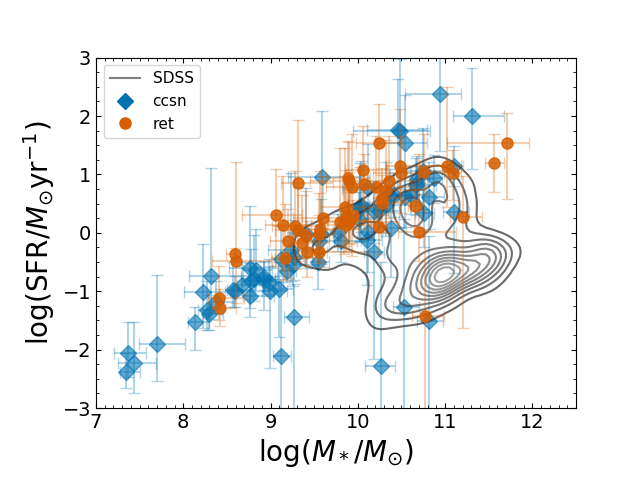
\includegraphics[width=0.5\textwidth]{figs/SFR_Mike.png}
\caption{The SFR of RET hosts, compared to CCSNe and the low-z SDSS sample.
\label{fig:sfms_sfr}}
\end{figure}

\begin{figure}
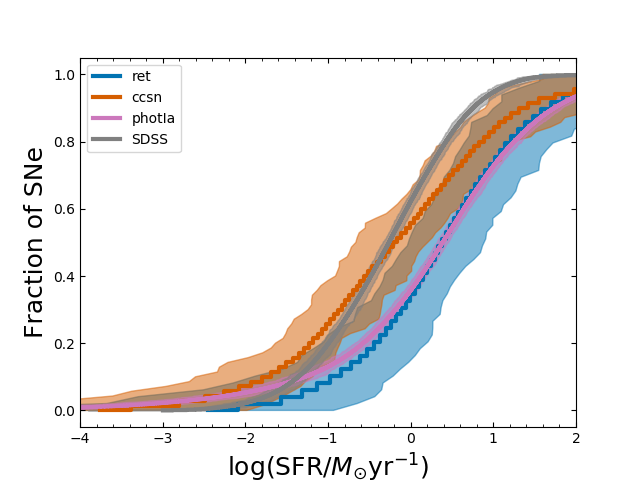
\includegraphics[width=0.5\textwidth]{figs/cum_SFR_mike.png}
\caption{Cumulative distributions of the SFR of RET hosts, compared to CCSNe and the low-z SDSS sample.
\label{fig:sfr_cum}}
\end{figure}
\subsection{Estimating metallicities \label{subsec:calc_Z}}

The most common method used to estimate the metallicity of galaxies is to use emission line ratios that have been calibrated using theoretical or empirical models in order to approximate the gas-phase oxygen abundance in the interstellar medium. Due to the low S/N of the spectra in this sample, we are constrained to a subset of these diagnostics by the availability of only a handful of the strongest emission lines, namely \halpha, \hbeta, \OII 3727, \OIII 4959 and 5007, \NII 6548 and 6583, and \SII 6717 and 6731. Furthermore, for each host galaxy only a subset of these lines are detected - for example, \halpha, \NII and \SII are redshifted out of the spectral coverage at $z>0.3$, leaving only the oxygen and \hbeta lines available, mandating the use of the R23 diagnostic. For hosts at $z<0.3$ we are able to use the \OIII /\NII (O3N2), \NII /\halpha (N2), and \SII /\NII (S2N2) line ratios. 

Due to the redshift range of our sample, and the limited wavelength coverage of the spectra ($3000-8000~\AA$), we are unable to use a single line ratio to estimate the oxygen abundances. We thus determine a set of indicators for which to calculate abundances. For the O3N2 and N2 indicators we use the calibration of \citet{Pettini2004} (PP04), and if \SII is detected we derive an abundance using the S2N2 diagnostic of \citet{Dopita2016}. For the R23 indicator, we use the calibration of \citet{Kobulnicky2004} (KK04). At abundances around $12 + \log \mathrm{(O/H)} \sim 8.4$, the R23 indicator becomes two-tailed, with a low and a high value of metallicity corresponding to a single R23 ratio. In cases where the lines are available, we break this degeneracy by cross-calibrating with the \NII / \OII ratio \citep{Kewley2008}. In the cases where \NII is not available, and there are no other diagnostics that can be used to inform the choice of branch, we use the host galaxy mass to derive a crude metallicity estimate from the MZR of \citet{Kewley2008} based upon the PP04 O3N2 diagnostic. For $12 + \log \mathrm{(O/H)}_{\mathrm{MZR}} < 8.4$ we chose the lower branch, while for higher MZR metallicities we choose the upper branch.

The samples to which we compare metallicities span different redshift ranges, were observed with different equipment, and in many cases were compiled before certain (particularly the D16) diagnostics were devised. Therefore, in order to compare oxygen abundances between different samples we transform all abundances onto the scale of PP04 (O3N2) using the conversion from \citet{Kewley2008}. This is not possible for the D16 diagnostic, so we discard it from the rest of our analysis, although for completeness we provide for DES RET hosts where available. For samples that quoted multiple diagnostics, or for which sufficient line flux measurements were provided from which to calculate multiple diagnostics, we calculate a weighted mean of the values after transforming them to the PP04 O3N2 scale.

\begin{figure}
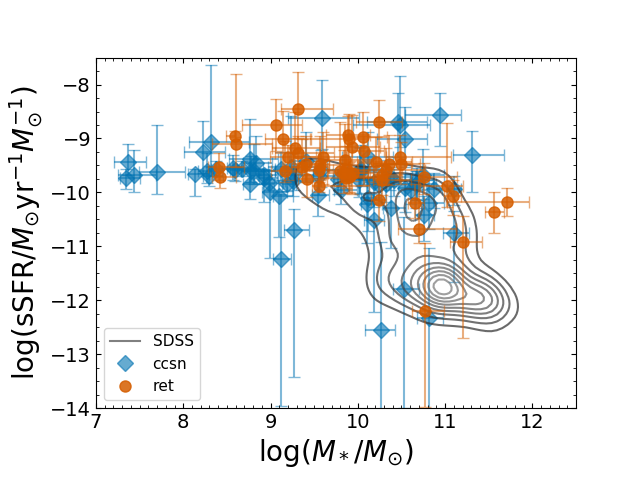
\includegraphics[width=0.5\textwidth]{figs/sSFR_Mike.png}
\caption{The sSFR of RET hosts, compared to CCSNe and the low-z SDSS sample.
\label{fig:sfms_ssfr}}
\end{figure}

\begin{figure}
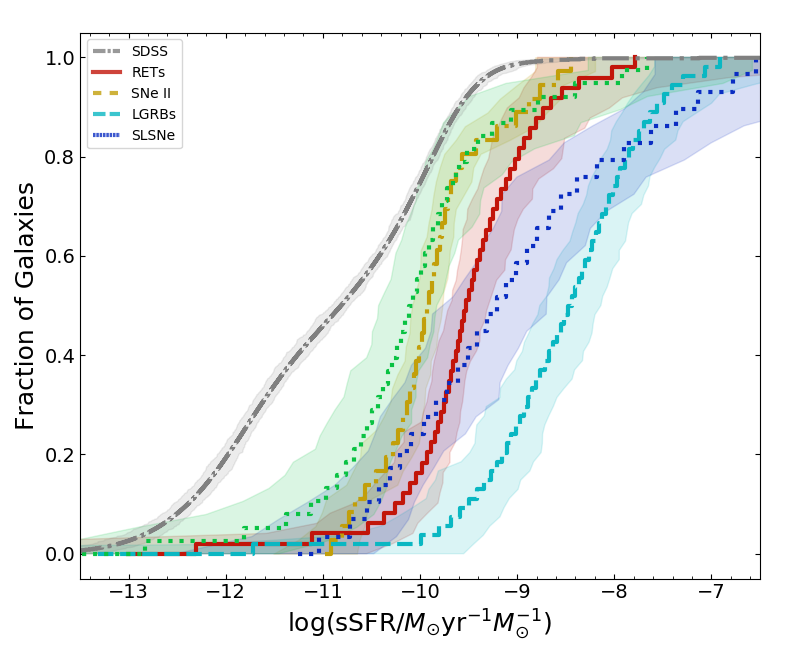
\includegraphics[width=0.5\textwidth]{figs/cum_sSFR_mike.png}
\caption{Cumulative distributions of the sSFR of RET hosts, compared to CCSNe and the low-z SDSS sample.
\label{fig:ssfr_cum}}
\end{figure}


\section{Analysis and Discussion}
\label{sec:analysis} % used for referring to this section from elsewhere



\subsection{Stellar Mass \label{subsec:res_mass}}

\subsection{Star formation rate \label{subsec:res_sfr}}
Fig.~\ref{fig:sfms_sfr} shows the `star formation main sequence' (SFMS) of RET host galaxies along with that for CCSNe and for the field galaxies of SDSS. RETs and CCSNe both systematically avoid passive galaxies, suggesting that RETs may require the presence of star-formation and thus be linked to massive stars.

In Fig.~\ref{fig:sfr_cum} we show the cumulative distributions of the star-formation rate in RETs, CCSNe, and SDSS galaxies. With the exception of three objects, all RETs occured in galaxies with $\textrm{SFR}>0.1 \msun$yr$^{-1}$, and the curve is shifted towards higher SFRs than that for CCSNe. This would imply that a higher SFR is required for RETs to occur - or can be thought of as a higher SFR threshold for the formation of a RET progenitor.

Fig.~\ref{fig:sfms_ssfr} is similar to Fig.~\ref{fig:sfms_sfr}, except that here SFR has been normalised by stellar mass, and thus shows the specific star-formation rate (sSFR), which is more representative measure of the star-forming intensity compared to galaxies of the same mass. It is once again clear that RET hosts lie systematically above the majority of SDSS star-forming galaxies. Normalised by mass, it is here perhaps clearer to see that RET hosts lie at higher sSFR than CCSNe hosts.

As for SFR, we show the cumulative distribution of sSFR in Fig.~\ref{fig:ssfr_cum}. The RET hosts are clearly shifted to higher sSFRs than CCSNe. To compare statistically the host sSFR distribution of RETs with the other samples, we employ the method of \citet{Wiseman2020}. For each pair of samples, we model the PDFs as skewed normal distributions. For both samples, we use identical normal priors for the `mean' and `scale'\footnote{See \citet{Wiseman2020} for a detailed description of the parameters describing the skewed normal distributions}, centred on the mean and twice the standard deviation of the two samples combined. 

\subsection{Metallicity \label{subsec:res_metallicity}}

\begin{figure}
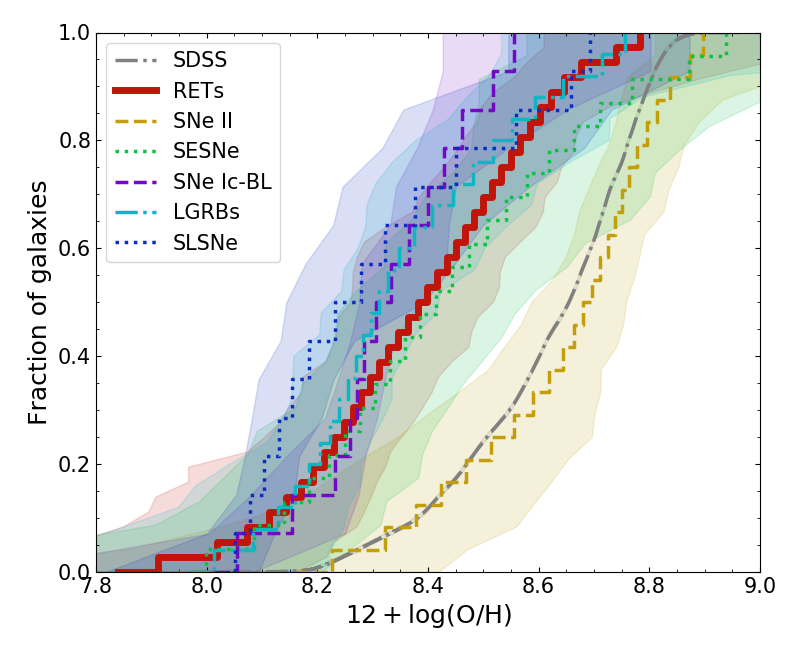
\includegraphics[width=0.5\textwidth]{figs/RET_OH_cum.png}
\caption{Cumulative distributions of the gas-phase oxygen abundances of RET hosts, compared to CCSNe and the low-z SDSS sample.
\label{fig:oh_cum}}
\end{figure}

\begin{figure}
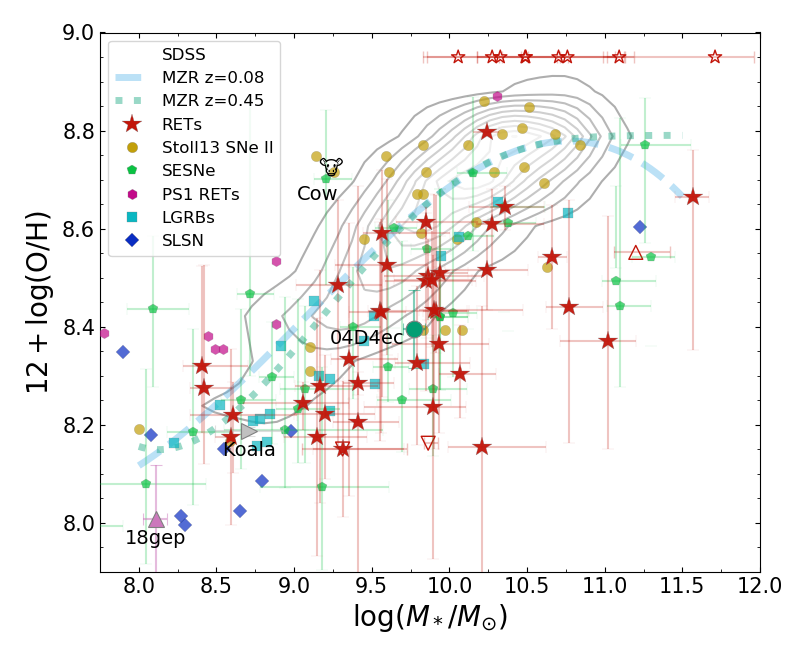
\includegraphics[width=0.5\textwidth]{figs/RET_MZR.png}
\caption{The mass-metallicity relation (MZR) for RET host galaxies.
\label{fig:mzr}}
\end{figure}


In the Section \ref{subsec:res_sfr} we demonstrate that RETs occur in galaxies with systematically higher sSFR than CCSNe, to which one explanation is that they are related to more massive stars. A further property that could directly impact the composition of stellar populations harbouring potential RET progenitors is the metallicity. Using the gas-phase oxygen abundances calculated in Section \ref{subsec:calc_Z} as a proxy for metallicity, we can compare the chemical state of RET host galaxies with CCSNe and star-forming field galaxies. The cumulative distributions of metallicity are displayed in \ref{fig:oh_cum}, and show RET hosts to be inconsistent with SNe II and field galaxies. The RET curve lies at lower metallicity than those galaxies, and appears visually similar to the curves for SESNe. RETs occur, on average, in slightly more metal-rich environments than LGRBs and SLSNe.

We compare the metallicity distributions in the same way as the sSFRs. The RET host metallicity distribution is significantly different to the SNe II and SDSS distributions, with no overlap in the posterior distributions for the skewed-normal distribution peak and skewness. On the other hand, simultaneous fits with SESNe show very similar distributions.

In Fig.~\ref{fig:mzr} we show the mass-metallicity relation (MZR) for the RET and comparison samples. The contours show the MZR for low-redshift ($\hat{z}=0.08$) star-forming galaixes from SDSS, adjusted to the PP04 O3N2 diagnostic. We use the MZR parameterisation \citet{Zahid2014} to show the best fit to the MZR for star-forming galaxies. The blue dashed line shows the fit to the low-z data, while the orange dashed line corresponds to the MZR at $z=0.45$, the mean redshift of the RET host sample. The RET hosts lie systematically below the galaxy MZR fits as well as the bulk of the SDSS galaxies, meaning that for a given stellar mass they have a lower metallicity.

\begin{figure}
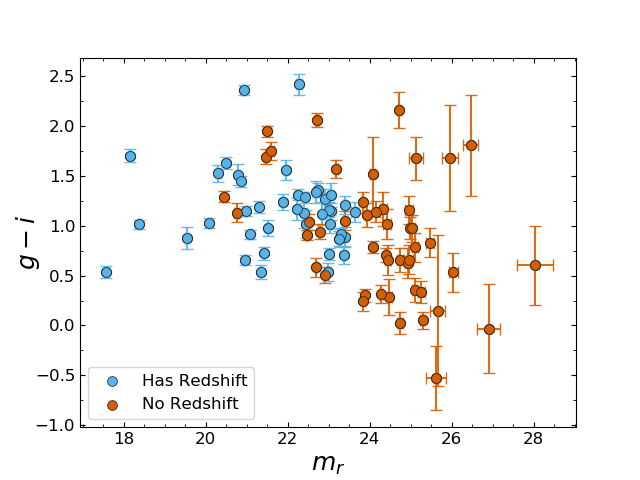
\includegraphics[width=0.5\textwidth]{figs/mag_v_colour.png}
\caption{The colour-magnitude distribution of RET hosts with (cyan) and without (orange) redshifts. There is an excess of objects with blue colours that do not have redshift measurements.
\label{fig:g-i}}
\end{figure}

\section{Discussion \label{sec:disc}}
\begin{figure}
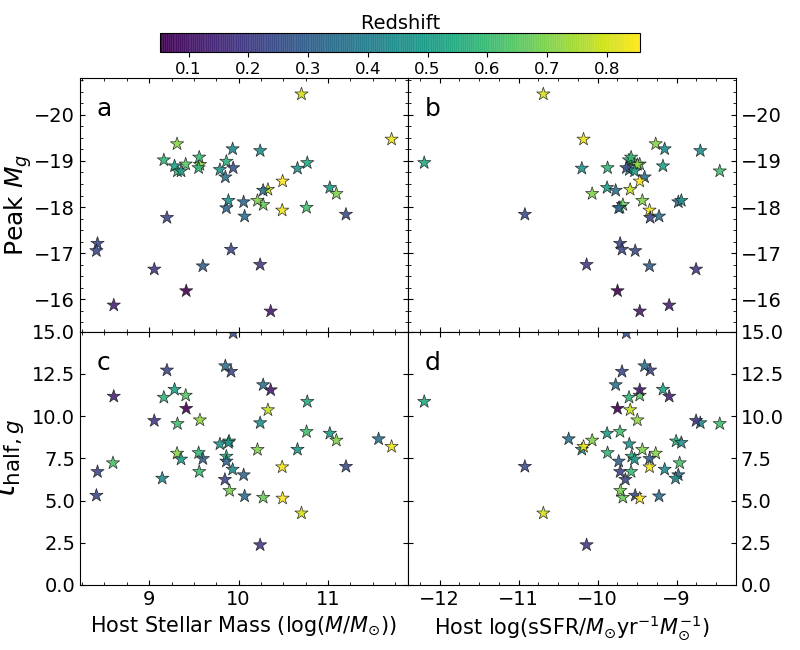
\includegraphics[width=0.5\textwidth]{figs/RET_vs_host.png}
\caption{RET lightcurve properties as a function of host galaxy measurements.
\label{fig:ret_v_host}}
\end{figure}
\subsection{Selection Biases \label{subsec:disc_bias}}
The properties presented in Section \ref{sec:analysis} are derived from a subset of the total sample of RETs. Of 106 objects, under half (49/106) have secure host galaxy redshifts. Three of these were obtained from transient spectra, for which we are unable to disentangle the host and transient contributions, and six were obtained by programmes for which we do not have access to the spectra. Of the remaining 42, it was possible to derive a metallicity for 37 host galaxies. The observed metallicity distribution could have arisen if the galaxies without redshifts (and metallicities) are systematically higher in metallicity than those for which measurements were possible. This scenario is unlikely. For low SNR objects, redshifts are typically obtained from only two of the strongest lines (e.g. \halpha, \hbeta, \OIII, and \OII), whose absolute luminosity is not strongly dependent on metallicity. It is likely that the redshifts were not obtained because of low SNR, caused by the galaxies being smaller and at higher redshift. We do not envisage a plausible scenario where those galaxies are systematically higher in metallicity.

Another possibility is that the hosts without a redshift are mostly non-starforming, passive galaxies, for which a redshift is typically harder to obtain than for emission-line galaxies \citep{Yuan2015,Childress2017,Lidman2020}. In order to test this possibility, we examined the RETs that do not have a host galaxy redshift. Table \ref{tab:z_cuts} shows the numbers of RETs that failed various stages of the redshifting process. Of the 48 objects without a redshift, 40 of them have host galaxies detected in the SN Deep coadds of \citet{Wiseman2020}. Of more significance is that only 34 have host galaxies in the SVA1 catalogues which were used for targetting during the OzDES campaign. The other, `hostless', objects are either transients that are located remotely from a host that was detected, or are hosted by a galaxy that was not detected. Non-detected hosts are either intrinsically faint and thus low in mass, situated at high redshift, or both. Neither are expected to be systematically higher in metallicity than the detected hosts. Similarly, a further 16 hosts were detected but not targetted by OzDES, due to being too faint to pass the selection criteria ($m_r < 24.5$), leaving 18 that were targetted but no redshift was found. The resulting redshift completeness of targetted objects is 70\% (82\% for objects brighter than $m_r = 24$~mag, which is in line with the average for OzDES as a whole \citep{Lidman2020}.
In Fig. \ref{fig:g-i} we show the observer-frame $r$-band magnitudes and $g-i$ colours for all RET hosts that were detected. The 40 objects with detected hosts but no redshift lie at fainter magnitudes, and appear to extend to bluer colours than those with secure redshifts. This is contrary to the hypothesis that they are high-redshift and/or passive hosts, but instead are low-mass, star-forming galaxies whose line fluxes were not strong enough to be detected.
 

\begin{table}
    \centering
    \begin{tabular}{l|l}
         Cut &  Number of remaining objects \\
        \toprule
        All RETs & 106 \\
        No redshift   & 48\\
        Host in SN Deep & 40\\
        Host in SVA1 & 34 \\
        Targetted by OzDES & 18 \\
        \bottomrule
    \end{tabular}
    \caption{Numbers of RETs passing various cuts relating to redshift targetting.}
    \label{tab:z_cuts}
\end{table}

\subsection{Origin of RETs}

The sample of DES RETs shows a preference for low-metallicity, strongly star-forming host environments. The PDF of their metallcities displays a strong similarity to the hosts of SNe Ibc, as well as LGRBs. There is a clear difference to the PDFs of SNe II, which follow SDSS field galaxies. The preference for low-metallicity systems is not as strong as for LGRBs or SLSNe, but the highest metallicities found in all three samples are very similar at around solar metallicity. This result is further suggestive of a stripped-envelope, massive-star origin for RETs. 
The population of RET hosts lies, on average, between CCSNe and LGRBs/SLSNe in terms of both star formation and metallicity. A loose correlation exists between the luminosity and rarity of events, and the host galaxy conditions required for their formation. The rough rate of RETs ($\geq 10^{-6} \mathrm{Mpc}^{-3} \mathrm{yr}^{-1}$), (\citetalias{Pursiainen2018}) is $\sim1\%$ of the CCSN rate \citep{Li2011,Horiuchi2011}, which itself is divided into the more common SNe II and sub-dominant SESNe \citep{Kelly2012,Frohmaier2020}. At $\sim1\%$ of the CCSN rate, RETs are more common than SLSNe ($\sim0.01 - 0.05\%$ of CCSNe; \citealt{McCrum2015,Prajz2016,Frohamier2020}) and LGRBs (intrinsically $\sim0.08\%$ when accounting for beaming; \citealt{Graham2016}). These figures place the DES RETs between extreme objects (SLSNe, LGRBs) and more common SNe (SNe II, SESNe) in terms of rate, matching their location in host galaxy parameter space. While stressing that these associations are lose - rates are uncertain and host galaxy parameters span wide ranges for all transients - they are both linked to the respective transients' progenitor channels. Based upon both indicators, it is reasonable to infer that RETs are linked to very massive stars that also require some extreme properties such as rapid rotation, albeit not as much as progenitors as SLSNe or LGRBs. It could therefore be possible that RETs are an intermediate and/or precursory step, whereby the initial collapse of the star occurs leading to a shocked photosphere, but conditions are not highly tuned enough for a LGRB or SLSN and the respective central engine does not form. 

\subsection{Correlations between lightcurve and host galaxy properties}
Many classes of transients show trends between properties intrinsic to the objects themselves and their host galaxies. For example, SNe Ia lightcurves appear to be broader in less massive galaxies with higher sSFR \citep{Sullivan2006,Neill2009,Howell2009,Sullivan2010,Roman2018,Kelsey2020}, while SLSNe that have been fit with a magnetar model show a tentative relationship between the magnetar spin period and host galaxy metallicity \citep{Chen2016a}. In Fig. \ref{fig:ret_v_host} we show the RET peak magnitude (upper pannels) and decline rate parameterised as $t_{\mathrm{half}}$, the time taken for the LC to decline to half the peak brightness (lower panels) and how they correspond to host galaxy stellar mass (left-hand panels) and sSFR (right-hand panels).

\section{Conclusions}

The last numbered section should briefly summarise what has been done, and describe
the final conclusions which the authors draw from their work.

\section*{Acknowledgements}

The Acknowledgements section is not numbered. Here you can thank helpful
colleagues, acknowledge funding agencies, telescopes and facilities used etc.
Try to keep it short.

%%%%%%%%%%%%%%%%%%%%%%%%%%%%%%%%%%%%%%%%%%%%%%%%%%

%%%%%%%%%%%%%%%%%%%% REFERENCES %%%%%%%%%%%%%%%%%%

% The best way to enter references is to use BibTeX:

\bibliographystyle{mnras}
\bibliography{PhilMendeley} % if your bibtex file is called example.bib


% Alternatively you could enter them by hand, like this:
% This method is tedious and prone to error if you have lots of references
%\begin{thebibliography}{99}
%\bibitem[\protect\citeauthoryear{Author}{2012}]{Author2012}
%Author A.~N., 2013, Journal of Improbable Astronomy, 1, 1
%\bibitem[\protect\citeauthoryear{Others}{2013}]{Others2013}
%Others S., 2012, Journal of Interesting Stuff, 17, 198
%\end{thebibliography}

%%%%%%%%%%%%%%%%%%%%%%%%%%%%%%%%%%%%%%%%%%%%%%%%%%

%%%%%%%%%%%%%%%%% APPENDICES %%%%%%%%%%%%%%%%%%%%%

\appendix

\section{Some extra material}

If you want to present additional material which would interrupt the flow of the main paper,
it can be placed in an Appendix which appears after the list of references.

%%%%%%%%%%%%%%%%%%%%%%%%%%%%%%%%%%%%%%%%%%%%%%%%%%


% Don't change these lines
\bsp	% typesetting comment
\label{lastpage}
\end{document}

% End of mnras_template.tex